% !TeX root = ../main-crpq-tw-lmcs.tex

\section{\AP{}Discussion}
\label{sec:discussion}

% Observe that the proof of our main theorem, \Cref{thm:decidability-semtw}, was divided into the upper-bound for $k \geq 2$ (\Cref{lem:sem-tw-in-twoexp}), the upper-bound for $k=1$ (\Cref{cor:sem-tw-1-pb-exp-c}), and the lower-bound for all $k$ (\Cref{lemma:lowerbound}). One could have proved the upper-bound for all $k$ by using "contracted tree-width" right from the beginning. But we preferred to keep things ``as simple as possible'' for the case $k \geq 2$ using the classical notion of "tree-width".

% \sidediego{I've added the related work section here. But I'm not married to the idea...}
% \subsection{\AP{}Related Work}
% \label{sec:relwork}
% The current paper is based on the conference paper \cite{FigueiraMorvan2023SemanticTreeWidthICDT}. While the main results are essentially the same, here we also show how to extend our techniques to tackle the "semantic tree-width $1$ problem" (\Cref{sec:acyclic-queries}) and we introduce and study the "semantic path-width $k$ problems" (\Cref{sec:semantic-path-width}).


% Barceló, Romero, and Vardi \cite[Theorem 6.1]{BarceloRomeroVardi2016SemanticAcyclicity} have studied the  "semantic tree-width $1$ problem" for "UC2RPQs" and shown that it is "ExpSpace"-complete. While their approach is in many ways different from ours, they also show the decidability by computing the "maximal under-approximation" of "tree-width" $1$ for "UC2RPQs". As it turns out, the "maximal under-approximation" of "UCRPQs" by "infinitary unions" of "CQs" of "tree-width" $1$ may not be expressible by a "UCRPQ" but rather by a "UC2RPQ". This is why the "semantic tree-width $1$@semantic tree-width $1$ problem" and the "\emph{one-way} semantic tree-width $1$ problems@one-way semantic tree-width $1$ problem" are different problems, and why they focused on the former.
% As we show, this difference between the one-way and two-way semantic problem is: (a) erased for "tree-width" $k$ as soon as $k>1$ ("cf" \Cref{thm:closure-under-sublanguages}) and (b) preserved for "path-width" $k$ for any $k$ ("cf" \Cref{rk:path-width:oneway-vs-twoway}).
% With our current approach, we can re-prove \cite[Theorem 6.1]{BarceloRomeroVardi2016SemanticAcyclicity}'s result and also obtain decidability for the "one-way semantic tree-width $1$ problem" ("cf" \Cref{cor:sem-tw-1-pb-exp-c}).


% On the class "conjunctive queries", the "semantic tree-width $k$ problem" becomes the "coNP"-complete problem of finding out whether the retraction of a query has "tree-width" at most $k$. Further, classes of "CQs" of bounded "semantic tree-width" precisely characterize tractable (fixed-parameter) "evaluation problem" \cite{Grohe2007ComplexityHomomorphism,DalmauKolaitisVardi2002Constraint}.\footnote{This result is on bounded-arity schemas, which was later generalized \cite{ChenGottlobLanzingerPichler2020Semantic} for characterizing "FPT" "evaluation" on arbitrary schemas ---by replacing "semantic tree-width" with semantic ``submodular width'' \cite{Marx13Tractable}.} The problem of computing "maximal under-approximations" of "CQs" of a given "tree-width" has been explored in \cite{BarceloLibkinRomero2014Efficient}. While "maximal under-approximations" of a given "tree-width" always exist for "CQs", this is not the case for the dual notion of ``minimal over-approximations''. The problem of when these exist is still unknown to be decidable, aside for some the special cases of acyclic "CQs" and Boolean "CQs" over binary schemas \cite{BarceloRomeroZeume2020Approximation}.


\subsection{\AP{}Complexity}
\label{sec:discussion-complexity}
We have studied the definability and approximation of "UC2RPQ" queries by queries of bounded "tree-width" and shown that the "maximal under-approximation" in terms of an infinitary union of "conjunctive queries" of "tree-width" $k$ can be always effectively expressed as a "UC2RPQ"
of "tree-width" $k$ (\Cref{cor:mua-exists-effective}). 
However, while the "semantic tree-width $1$ problem" is shown to be "ExpSpace"-complete (which was also established in \cite[Theorem 6.1, Proposition 6.2]{BarceloRomeroVardi2016SemanticAcyclicity}), we have left a gap between our lower and upper bounds in \Cref{thm:decidability-semtw} for every $k>1$.

\begin{question}
    For $k > 1$, is the "semantic tree-width $k$ problem" "ExpSpace"-complete?
\end{question}
A related question is whether the "containment problem" between a "C2RPQ" and a "summary query" is in "ExpSpace". Should this be the case, then the "semantic tree-width $k$ problem" would be in "ExpSpace".
We also point out that since every "path-$l$ approximation" can be expressed by a polynomial "UC2RPQ" of tree-width $2k$---this is the same idea as in \cite[Lemma IV.13]{RomeroBarceloVardi2017Homomorphism}---, one can produce, for every "UC2RPQ" $\Delta$ a union $\Gamma$ of poly-sized "C2RPQ" of tree-width $2k$ such that $ \MUA{\Delta}{\Tw} \contained \Gamma \contained \Delta$. This implies that the following ``promise'' problem\footnote{In reference to ``promise constraint satisfaction problems''
\cite[Definition 2.3]{BrakensiekGuruswami2021PCSP}.} is decidable in "ExpSpace": given a "UC2RPQ" $\Gamma$, answer `yes' if $\Gamma$ is of "semantic tree-width" $2k$, and answer `no' if $\Gamma$ is not of "semantic tree-width" $k$. The fact that $\MUA{\Delta}{\Tw}$ can be approximated by an exponential query of tree-width $2k+1$ can also be seen as a corollary of the proof of \cite[Theorem~V.1]{RomeroBarceloVardi2017Homomorphism}.

We also do not know whether the {"PiP2"} bound on the "semantic tree-width $k$ problem" for {\UCRPQSRE} has a matching lower bound. The known lower bound for the {\UCRPQSRE} "containment problem" \cite[Theorem~5.1]{FigueiraEtal2020Containment} does not seem to be useful to be employed in a reduction in this context, since it necessitates queries of arbitrary high "tree-width".

\subsection{\AP{}Characterization of Tractability}
\label{sec:charact-tractability}

Our result implies that for each $k$
the "evaluation problem" for "UC2RPQs" $\Gamma$
of "semantic tree-width" $k$ is "fixed-parameter tractable" when parametrized
by the size of the query, "ie" it works in time $\+O(|G|^{c} \cdot f(|\Gamma|))$
for a computable function $f$ and constant $c$, where $G$ is the "database@@graph" given as input.
%
While this was a known fact \cite[Corollary IV.12]{RomeroBarceloVardi2017Homomorphism}, the dependence on the database was $c=2k+1$.  Our results show that the dependence can be improved to $c=k+1$, similarly to \cite[Theorem 6.3]{BarceloRomeroVardi2016SemanticAcyclicity} for the case $k=1$.
It has been further shown by Feier, Gogacz and Murlak that the "evaluation" can be done with a single-exponential $f$ \cite[Theorem~22]{FeierGogaczMurlak24Treewidth}.
% This improves the dependence on the size of the database,
% namely $\+O(|G|^{2k+2} \cdot f(|\Gamma|))$, proven by
% Romero, Barceló and Vardi \cite[Corollary IV.12]{RomeroBarceloVardi2017Homomorphism}.

In a similar vein, our results show that the "evaluation problem" for "UC2RPQs"
of "semantic path-width" $k$ is in "para-NL". It is unknown whether the semantic bounded width properties characterize all "FPT" and "para-NL" classes.

\begin{question}\AP\label{qu:paraNLtractability}
    Does every recursively enumerable class of "CRPQs" with "para-NL" evaluation have bounded "semantic path-width"?
\end{question}

\begin{question}[Also mentioned in {\cite[\S IV-(4)]{RomeroBarceloVardi2017Homomorphism}}]\AP\label{qu:FPTtractability}
    Does every recursively enumerable class of "CRPQs" with "FPT" evaluation have bounded "semantic tree-width"?
\end{question}

Note that the classes of bounded "contracted path-width" or "contracted tree-width" are not counterexamples to \Cref{qu:paraNLtractability,qu:FPTtractability}, since
the "path-width" is upper-bounded by one plus the "contracted path-width", and lower-bounded by the "contracted path-width"---and similarly for "tree-width"---and so a width is bounded "iff" its "contracted" variant is bounded.

In the case of "CQs", the answer is `yes' to \Cref{qu:FPTtractability} \cite[Theorem~1]{Grohe2007ComplexityHomomorphism}
under standard complexity-theoretic hypotheses ($W[1] \neq $ "FPT"). For \Cref{qu:paraNLtractability}, the answer is still `yes' \cite[Theorem 3.1]{ChenMoritz13} conditional to a less standard assumption\footnote{By \cite[Theorems 3.1 \& 4.3]{ChenMoritz13}, if the class has bounded "semantic path-width", then the problem is in $\textsf{Path} \subseteq $ "paraNL"; by \cite[Theorems 3.1 \& 5.5]{ChenMoritz13}, if the class does not have bounded "semantic path-width", then the problem is \textsf{Tree}-hard.} (no $\textsf{Tree}$-hard problem is in "paraNL").

However, attempting at answering these questions for "CRPQs" is considerably more challenging. In particular, one important technical difficulty is that a class of "CRPQs" with unbounded "tree-width" may contain queries with no "expansions" which are "maximal" in the sense of "containment". That is, for every $k$, for every query $\gamma$ of "semantic tree-width" $>k$ and "expansion" $\xi$ of "semantic tree-width" $>k$ there may be another "expansion" $\xi'$ such that $\xi' \homto \xi$ ("ie", such that $\xi \contained \xi'$).  
% This brakes the reduction shown for "CQs" in \cite[Theorem~4.1]{Grohe2007ComplexityHomomorphism}. 
In fact, for classes of "CRPQs" avoiding such problematic behavior, Question~\ref{qu:FPTtractability} can be positively answered. We next show why.

\AP
Let us call a "UC2RPQ" ""finitely-redundant"" if there is no infinite chain $\xi_1(\bar x) \strcontained \xi_2(\bar x) \strcontained \dotsb$ among its "expansions". See \Cref{fig:example-infinite-chain} for a non-example.
\begin{figure}
    \centering%
    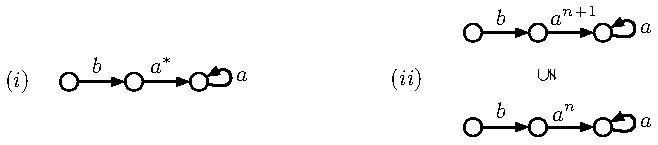
\includegraphics[width=.7\linewidth]{example-infinite-chain.pdf}
    \caption{%
        \AP\label{fig:example-infinite-chain}%
        $(i)$ A simple non-"finitely-redundant" Boolean "CRPQ". $(ii)$ For every $n$, there is a "homomorphism" from the $(n+1)$-"expansion" to the $n$-"expansion", but no "homomorphism" in the converse direction.
    }
\end{figure}
\AP
Observe that the classes of "CQs" and "UCQs" are "finitely-redundant", and also the class of ""loopless CRPQs"", meaning no directed cycle in its underlying directed graph and no empty word $\varepsilon$ in the "atom" languages.

\begin{lemma}
    The class of "loopless CRPQs" is "finitely-redundant".
\end{lemma}
\begin{proof}
    By means of contradiction, let $\gamma$ be "loopless" and suppose there is an infinite chain $\xi_1(\bar x) \strcontained \xi_2(\bar x) \strcontained \dotsb$ of "expansions" of $\gamma$. Hence, there must be an "atom" "expansion" which grows arbitrarily in the chain. Take $\xi_i$ such that it contains an "atom" "expansion" of size bigger than $\xi_1$. Since such "atom" "expansion" is a directed path (as we are dealing with one-way "CRPQs"), the fact that $\xi_i \homto \xi_1$ implies that there is some cycle in $\xi_1$.
    Since $\gamma$ cannot contain the empty word in the "atom" languages, this is in contradiction with the hypothesis that there are no "directed cycles" in $\gamma$.
\end{proof}

We next show that, restricted to classes of "finitely-redundant" "UC2RPQ", we can obtain a characterization of "evaluation" in "FPT".
\thmtractabilityfinred
\begin{proof}
    \proofcase{Left-to-right} By contraposition, we show that if $\+C$ has unbounded "tree-width", then its "evaluation problem" is "W[1]"-hard via an "FPT"-reduction from the 
    \AP
    ""parameterized clique problem"". This is the problem of, given a parameter $k$ and a simple graph $G$, whether $G$ contains a $k$-clique. We do this by a simple adaptation of the proof of Grohe \cite[Theorem~4.1]{Grohe2007ComplexityHomomorphism} for the case of "CQs".

    Given an instance $\langle G,k \rangle$ of the "parameterized clique problem", the idea is to first search for a query $\gamma \in \+C$ of ``sufficiently large'' "semantic tree-width". 
    
    \todo{update this shit}
    \AP
    Let us call an "expansion" $\xi$ of a "UC2RPQ" to be ""maximal"" if there is no other "expansion" $\xi'$ such that $\xi \strcontained \xi'$.
    \AP
    Recall that the "core" of a "CQ" is the result of repeatedly removing any atom which results in an equivalent query. It is unique up to isomorphism---see ---, and a "CQ" has "semantic tree-width" $k$ if{f} its "core" has "tree-width" $k$ \cite[Theorem 12]{DalmauKolaitisVardi2002Constraint}. We say that a "CQ" is `a core' if it is isomorphic to its "core".

    \begin{proposition}
        \label{prop:big-expansion}
        For any $k \geq 3$, if a "finitely-redundant" "C2RPQ" has "semantic tree-width" $\geq k$, then there is a "maximal" "expansion" thereof of "semantic tree-width" $\geq k$.
    \end{proposition}

    \begin{proof}
        Let $\gamma$ be a "finitely-redundant" "C2RPQ".
        Consider the "infinitary UCQ" \[\Xi \defeq \{\core{\xi} \mid \xi \text{ is a "maximal" "expansion" of } \gamma \}.\]
        Since $\gamma$ is "finitely-redundant", we have $\gamma \semequiv \Xi$.
        We prove the fact by contraposition.
        If all "maximal" "expansions" of $\gamma$ have "semantic tree-width" $\leq k-1$,
        then all "CQs" of $\Xi$ have "tree-width" $\leq k-1$, and so
        by the implication $\itemClosureInfCQ \Rightarrow \itemClosureUCRPQSimple$ of \Cref{thm:closure-under-sublanguages}, query $\gamma$ has "semantic tree-width" at most $k-1$.
        Note that for \Cref{thm:closure-under-sublanguages} to apply, we need $k-1 > 1$
        "ie" $k \geq 3$.
    \end{proof}

    \begin{proposition}
        The set of all "maximal" "expansions" of queries from $\+C$ is recursively enumerable.
    \end{proposition}

    \begin{proof}
        \AP We first show that given an "expansion" $\xi$ of some "C2RPQ" $\gamma$, it is 
        decidable whether $\xi$ is "maximal". This follows from the following claim:
        there exists an "expansion" $\xi'$ of $\gamma$ "st" $\xi' \homto \xi$ and
        $\xi \nothomto \xi'$ "iff"
        there exists such an "expansion" whose "atom expansions" have length at most
        $2^m \cdot |\xi|\cdot |\A|^{2|\xi|}$ where $|\xi|$ is the number of variables of $\xi$ and
        $m$ is the greatest number of states of an NFA labelling an "atom" of $\gamma$. 
        Decidability of "maximality" clearly follows from this claim: it suffices to check if 
        $\xi' \homto \xi$ implies $\xi \homto \xi'$ for all ``small'' $\xi'$.

        To prove the claim, let $\xi'$ be an "expansion" of $\gamma$, and assume that there is 
        a homomorphism $f\colon \xi' \to \xi$ and that $\xi \nothomto \xi'$. Consider an "atom expansion"
        \[
            \pi' = x_0 \atom{a_1} x_1 \atom{a_2} \cdots \atom{a_{n-1}} x_{n-1} \atom{a_n} x_n
        \]
        of $\xi'$, and let $\+A$ denote the NFA associated with the "atom".
        For any index $i \in \lBrack 0,n\rBrack$ which is neither among the $|\xi|$ first positions
        nor the $|\xi|$ last positions, define its type $\tau_i$ as
        the word $a_{i-|\xi|}-1 \cdots a_i a_{i+1} \cdots a_{i+|\xi|}$ of length $2|\xi|$---note that $\tau_i$ uniquely describes the ball of radius $|\xi|$ centred at $x_i$ in $\xi$.
        Consider the function which maps index $i \in \lBrack |\xi|, n-|\xi|+1\rBrack$
        to the pair $\langle f(x_i), Q_i , \tau_i \rangle$, where $Q_i$ is the set of states $q$
        of $\+A$ which admit a path from an initial state to $q$ labelled by $a_1\cdots a_i$.
        If $n \geq |\xi|\cdot 2^{|\+A|}\cdot |\A|^{2|\xi|} + 2|\xi|$ then by the pigeon-hole principle,
        there exists $i,j \in \lBrack |\xi|, n-|\xi|+1\rBrack$ "st" $i<j$, $f(x_i) = f(x_j)$,
        $Q_i = Q_j$ and $\tau_i = \tau_j$. Letting
        \[
            \pi'' = x_0 \atom{a_1} x_1 \atom{a_2} \cdots \atom{a_{i-1}} x_{i-1} \atom{a_i} x_i = x_j
            \atom{a_{j+1}} x_{j+1} \atom{a_{j+2}} \cdots \atom{a_{n-1}} x_{n-1} \atom{a_n} x_n,
        \]
        consider the query $\xi''$ obtained from $\xi'$ 
        by replacing $\pi'$ with $\pi''$.
        Since $Q_i = Q_j$, $\xi''$ is still an "expansion" of $\gamma$.
        Moreover, $f(x_i) = f(x_j)$ implies that there is a "homomorphism" from $\xi''$ to $\xi$.
        Lastly, it there was a "homomorphism" from $\xi$ to $\xi''$,
        then this homomorphism should contain $x_i$ in its image---otherwise there would clearly be a "homomorphism" from $\xi$ to $\xi'$. Note that the image of this "homomorphism"
        is included in the ball of $\xi''$ centered at $x_i = x_j$ of radius $|\xi|$.
        But since $\tau_i = \tau_j$ this ball is equal to the ball of $\xi'$ centered at $x_i$
        (or equivalently at $x_j$) of radius $|\xi|$, and so we found a "homomorphism" from
        $\xi$ to $\xi'$, which is not possible. Hence, there cannot be any "homomorphism" from
        $\xi$ to $\xi''$, which concludes the proof.

        Finally, to enumerate all "maximal" "expansions" of queries from $\+C$,
        it suffices to enumerate all "expansions" of queries from $\+C$---which is doable since $\+C$ is recursively enumerable---and only keep those which are "maximal", using the previous algorithm.
    \end{proof}

    We proceed with the reduction.
    For any value of $k$ which is big enough, we enumerate all "maximal" "expansions" of $\+C$ until we find one such "expansion" $\xi$ whose "core" contains a $K \times K$ grid as a minor, for $K = {k \choose 2}$.
    We know that this must happen by \Cref{prop:big-expansion} and the Excluded Minor Theorem \cite{RobertsonSeymour1986GraphMinors5}, stating that there exists a function $f : \N \to \N$ such that for every $n \in \N$ every graph of "tree-width" at least $f(n)$ contains a $(n \times n)$-grid as a minor.
    Once we get hold of such a "maximal" "expansion" $\xi$, we proceed as in \cite[proof of Theorem~4.1]{Grohe2007ComplexityHomomorphism} to produce, in polynomial time, a "graph database" $G_\xi$ such that:
    \begin{enumerate}
        \item there is a "homomorphism" $G_\xi \homto \xi$, and
        \item $G_\xi$ "satisfies@@db" $\xi$ if, and only if, $G$ has a clique of size $k$.
    \end{enumerate}
Now consider the "UC2RPQ" $\Gamma \in \+C$ of which $\xi$ is an expansion, and observe that if $G_\xi$ "satisfies@@db" $\Gamma$, then we must have that $G_\xi$ also "satisfies@@db" $\xi$, by the fact that $G_\xi \homto \xi$ and $\xi$ is "maximal". Hence, the following are equivalent:
\begin{itemize}
    \item $G_\xi$ "satisfies@@db" $\Gamma$, 
    \item $G_\xi$ "satisfies@@db" $\xi$,
    \item $G$ contains a $k$-clique.
\end{itemize}
This finishes the "FPT"-reduction.

\medskip

\proofcase{Right-to-left} This direction does not need any of the hypotheses (neither "finite-redundancy",  $"W[1]" \neq $ "FPT", nor r.e.), by \Cref{coro:fpt-eval-bounded-semtreewidth}.
\end{proof}

\subsection{\AP{}Larger Classes}
\label{sec:discussion-larger-classes}

A natural and simple approach to extend the expressive power of "CRPQs" is to close the queries by transitive closure. That is, given a binary "CRPQ" $\gamma(x,y)$ we can consider "CRPQ" over the extended alphabet $\A \cup \set \gamma$, where the label $\gamma$ is interpreted as the binary relation defined by $\gamma(x,y)$. \AP This is the principle behind ""Regular Queries"" \cite{ReutterRomeroVardi2017RegularQueries}. The notion of "tree-width" can be easily lifted to this class, and classes of bounded "tree-width" still have a polynomial-time "evaluation problem". However, this class has not yet been studied in the context of the "semantic tree-width". It is not known if the "semantic tree-width $k$ problem" is decidable, nor whether classes of bounded "semantic tree-width" have an "FPT" "evaluation problem".
\begin{question}
    Is the "semantic tree-width $k$ problem" for "Regular Queries" decidable?
\end{question}

\subsection{\AP{}Different Notions}
\label{sec:discussion-different-notions}

\begin{table}[bht]
    \begin{tabular}{ccc}
        \toprule
        Query class & Membership problem & "Evaluation problem" \\ \midrule
        "path-width" $\leq k$ & 
        "L"-c {\footnotesize\cite[Theorem 1.3, p. 2]{KintaliMunteanu2010Computing}}
        & "NL"-c {\footnotesize(\Cref{lemma:evaluation-bounded-pathwidth})}  \\
        "sem. path-w." $\leq k$ & "2ExpSpace" \& "ExpSpace"-h & "paraNL" {\footnotesize(\Cref{thm:evaluation-bounded-pathwidth})} \\ 
        & {\footnotesize(\Cref{thm:decidability-sempw})} \\ \midrule
        "tree-width" $\leq k$ & "L"-c {\footnotesize \cite[Lemma 1.4]{ElberfeldJakobyTantau2010Logspace}} & "P" {\footnotesize(Folklore)\footnotemark} \\
        "sem. tree-w." $\leq k$ & "2ExpSpace" \& "ExpSpace"-h\footnotemark & "FPT" {\footnotesize\cite[Corollary V.2]{RomeroBarceloVardi2017Homomorphism}}\footnotemark \\
        & {\footnotesize(\Cref{thm:decidability-semtw})} & "NP"-c {\footnotesize\cite[Theorem V.3]{RomeroBarceloVardi2017Homomorphism}}\\ \bottomrule
    \end{tabular}
    \caption{
        \label{table:tractability-classes-queries}
        Complexity of the membership and "evaluation problem" for
        some classes of "UC2RPQs" studied in this chapter, where $k \geq 1$ is fixed.
        The same results hold for the "contracted" variants.
        The abbreviation ``-c'' (resp. ``-h'') stands for ``-complete'' (resp. ``-hard'').
    }
\end{table}
\addtocounter{footnote}{-2}
\footnotetext{Originally proven by Chekuri \& Rajaraman \cite[Theorem 3]{ChekuriRajaraman2000Containment} for CQs. The generalization to "UC2RPQs" is trivial, see "eg" \Cref{prop:crpq-bound-tree-width-upper-bound}
or \cite[Theorem IV.3]{RomeroBarceloVardi2017Homomorphism}.}
\stepcounter{footnote}
\footnotetext{See also \cite[Theorem 6.1]{BarceloRomeroVardi2016SemanticAcyclicity} for $k=1$.}
\stepcounter{footnote}
\footnotetext{See also \Cref{coro:fpt-eval-bounded-semtreewidth} and \cite[Theorem~22]{FeierGogaczMurlak24Treewidth}.}


"CRPQs" of small "tree-width" or "path-width" enjoy a tractable "evaluation problem", see \Cref{table:tractability-classes-queries}. However, it must be noticed that "containment" between "tree-width" $k$ or "path-width" $k$ queries is still very hard: "ExpSpace"-complete (even for $k=1$) \cite{CalvaneseDeGiacomoLenzeriniVardi2000Containment}. The more restrictive measure of ``"bridge-width"'' \cite{Figueira2020Containment} has been proposed as a more robust measure, which results in classes of queries which are well-behaved both for "evaluation" (since "bridge-width" $k$ implies "tree-width" $\leq k$) and for "containment" (since "containment" of bounded-"bridge-width" classes is in "PSpace").
It is not hard to see that "bridge-width" is closed under "refinements", and thus that this notion is amenable to our approach ("cf" \Cref{obs:equivalence_under_approx_homomorphism}).
\begin{question}
    \AP\label{qu:semantic-bridge-width}
    Is the problem of whether a "UC2RPQ" is equivalent to a "UC2RPQ" of "bridge-width" at most $k$ decidable?
\end{question}